\documentclass[12pt]{report}
\usepackage[left=2.5cm,right=2.5cm,top=3cm,bottom=3cm]{geometry}
\usepackage{fancyhdr}
\usepackage{etoolbox}
\usepackage{titlesec}
\usepackage{titling} 
\usepackage{pgfplots}

\pagestyle{fancy}
\fancyhf{} 
\fancyhead[L]{UTN-FRC}
\fancyhead[C]{FISICA ELECTRONICA: TPL1}
\fancyhead[R]{2R3}
\renewcommand{\headrulewidth}{0.4pt}
\fancyfoot[C]{\vfill\thepage}

\patchcmd{\chapter}{\thispagestyle{plain}}{\thispagestyle{fancy}}{}{}

%\renewcommand{\chaptername}{Experiencia}

\titleformat{\chapter}[display]
  {\normalfont\huge\bfseries}{\chaptertitlename\ \thechapter}{20pt}{\huge}
\titlespacing*{\chapter}{0pt}{0pt}{0pt}

\DeclareMathSizes{12}{13}{6}{5}

\title{%
  \fontsize{25}{0}\selectfont Universidad Tecnológica Nacional \\
  \fontsize{22}{30}\selectfont Física 2 \\
  \fontsize{18}{25}\selectfont TPL1: Calorimetría
}
\author{
Franco Palombo\\
Gaston Grasso\\
Ignacio Gil\\
Luciano Cortesini\\
}
\date{03 / 10 / 2024}

\begin{document}

\chapter{Introduccion}
  El fenomeno de la radiacion es la propagacion de energia en forma de ondas electromagneticas o particulas subatomicas
  que viajan a traves del vacio o de un medio en especifico.\\

  Existen multiples tipos de radiacion, pero para el enfoque de este trabajo practico, se va a experimentar con la
  radiacion electromagnetica a partir de una fuente de luz infrarroja, como puede ser la emitida por cualquier cuerpo
  que se encuentra a una temperatura mayor a 0ºK y mayor a la del entorno en donde se encuentra. Este tipo de radiacion
  es denominada radiacion termica. Es producto del movimiento termico que presentan las particulas cargadas presentes
  en la materia. La intensidad de esta radiacion depende de la temperatura de la materia o el cuerpo y de la longitud
  de onda que se considere.\\

  Los cuerpos pueden ser emisores de radiacion o receptores de radiacion. En ambos casos, las cantidades son iguales,
  pero opuestas. Esto es debido a reciprocidad, un fenomeno que establece que la razon de emision de radiacion
  electromagnetica de un cuerpo a una frecuencia dada, va a ser la misma a la que el cuerpo pueda absorber.\\

  Para cuerpos emisores, la intensidad de la radiacion emitida, puede propagarse en cualquier direccion en cualquiera
  de sus superficies o caras. Asimismo, la emisividad de un cuerpo es la razón entre la intensidad emitida por la
  superficie en una dirección particular y la intensidad que sería emitida por un cuerpo negro a la misma temperatura y
  longitud de onda.\\

  Existe un tipo de cuerpo, cuyas capacidades de emision y absorcion son ideales. Este cuerpo, denominado cuerpo negro,
  esta caracterizado por permitir el paso de todos las ondas electromagneticas, independientemente de su longitud de
  onda o su direccion. Tambien, no hay superficie que pueda emitir mas radiacion que la de un cuerpo negro en las
  mismas condiciones de temperatura y longitud de onda.\\

  Habiendo presentado estos conceptos, se procede a presentar las experiencias de laboratorio.

\chapter{Experiencia de laboratorio}
  Esta experiencia consta en la utilizacion del cubo de Leslie, un dispositivo que contiene en su interior una fuente
  de radiacion termica en forma de una bombilla incandescente. Una caja metalica, colocada sobre la bombilla, se pone
  en contacto con diferentes tipos de materiales, para probar dos propiedades de los mismos:
  \begin{itemize}
    \item Capacidad de emision
    \item Capacidad de absorcion
  \end{itemize}

  Estas propiedades permiten caracterizar diferentes materiales como aislantes o conductores termicos, y dependiendo de
  diferentes propiedades fisicas, se los puede emplear como capas protectoras del calor o instrumentos de dispersion de
  calor.

%aluminio temp vs tiempo
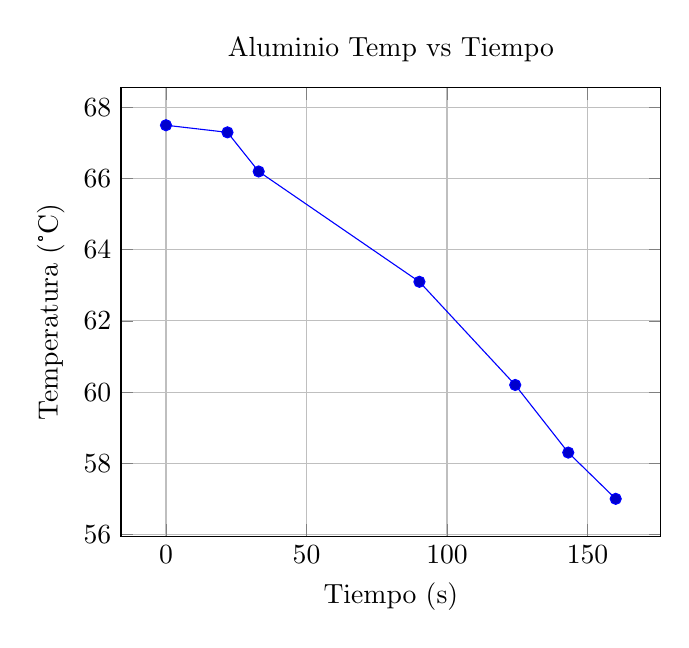
\begin{tikzpicture}
    \begin{axis}[
        xlabel={Tiempo (s)},
        ylabel={Temperatura (°C)},
        title={Aluminio Temp vs Tiempo},
        grid=major,
        legend pos=north west % Posición de la leyenda
    ]
    % Primera función
    \addplot coordinates {
      (0,67.5) (21.87,67.3) (32.98,66.2) (90.17,63.1) (124.26,60.2) (143.13,58.3) (160.01,57)
    };
    \end{axis}
\end{tikzpicture}
%aluminio rad vs tiempo
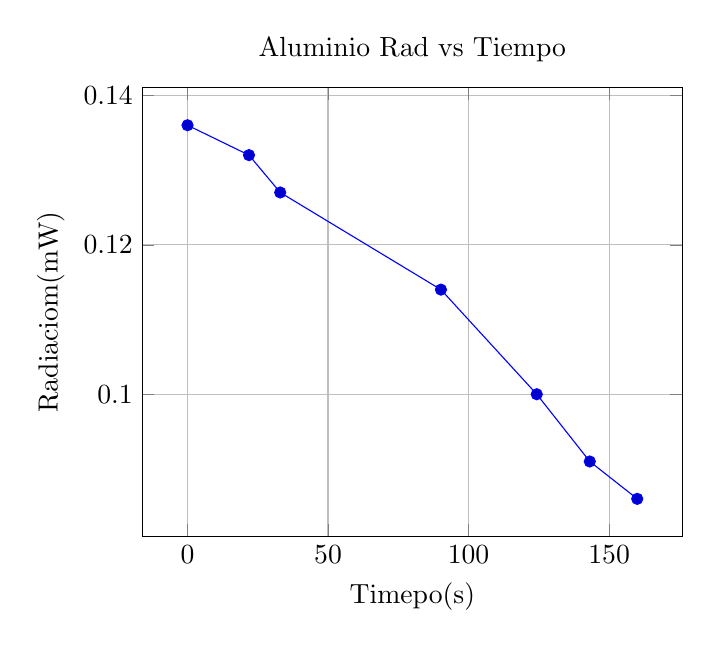
\begin{tikzpicture}
    \begin{axis}[
        xlabel={Timepo(s)},
        ylabel={Radiaciom(mW)},
        title={Aluminio Rad vs Tiempo},
        grid=major,
        legend pos=north west 
    ]
    \addplot coordinates {
    (0,0.136) (21.87,0.132) (32.98,0.127) (90.17,0.114) (124.26,0.1) (143.13,0.091) (160.01,0.086)
    };
    \end{axis}
\end{tikzpicture}\\
%bronce temp vs tiempo
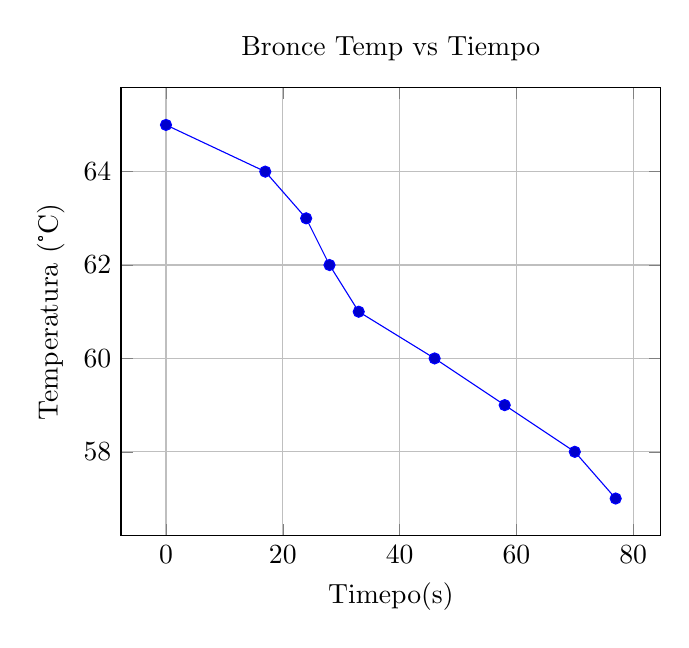
\begin{tikzpicture}
    \begin{axis}[
        xlabel={Timepo(s)},
        ylabel={Temperatura (°C)},
        title={Bronce Temp vs Tiempo},
        grid=major,
        legend pos=north west
    ]
    \addplot coordinates {
      (0,65) (17,64) (24,63) (28,62) (33,61) (46,60) (58,59) (70,58) (77, 57)
    };
    \end{axis}
\end{tikzpicture}
%bronce rad vs tiempo
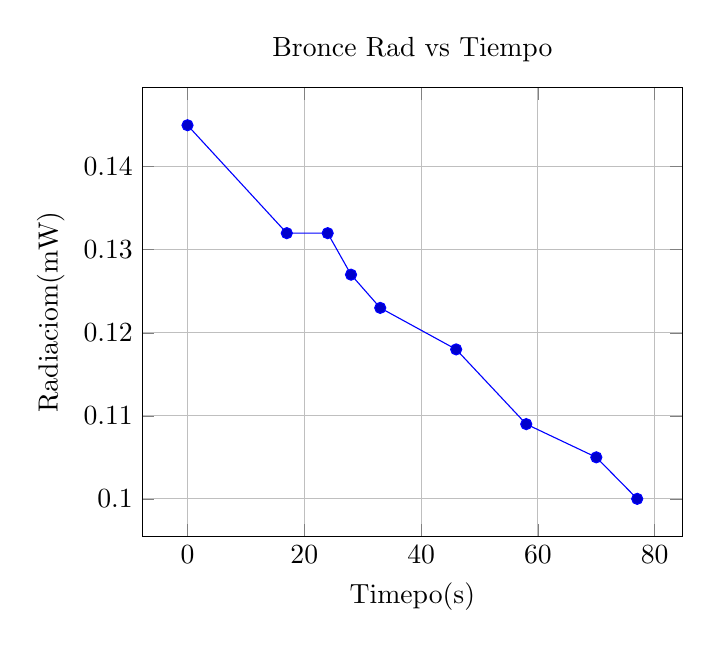
\begin{tikzpicture}
    \begin{axis}[
        xlabel={Timepo(s)},
        ylabel={Radiaciom(mW)},
        title={Bronce Rad vs Tiempo},
        grid=major,
        legend pos=north west
    ]
    \addplot coordinates {
      (0,0.145) (17,0.132) (24,0.132) (28,0.127) (33,0.123) (46,0.118) (58,0.109) (70,0.105) (77, 0.1)
    };
    \end{axis}
\end{tikzpicture}\\


%Plomo Temp vs tiempo
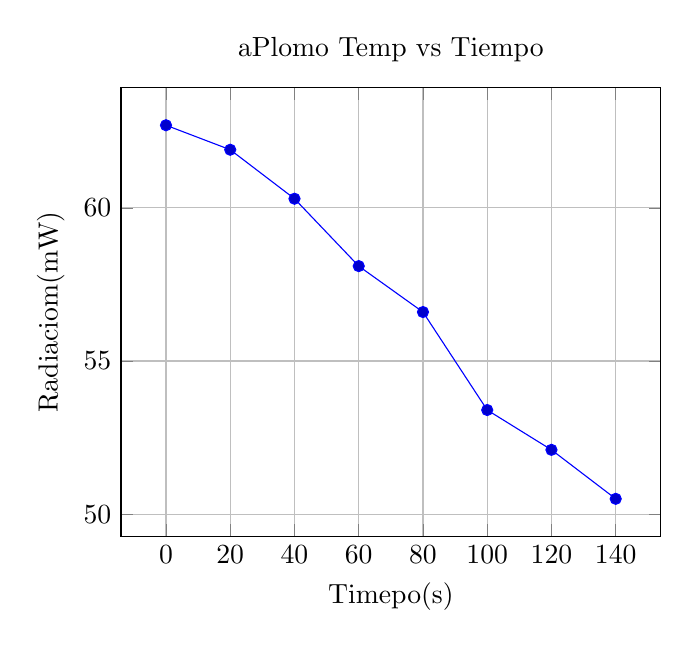
\begin{tikzpicture}
    \begin{axis}[
        xlabel={Timepo(s)},
        ylabel={Radiaciom(mW)},
        title=a{Plomo Temp vs Tiempo},
        grid=major,
        legend pos=north west
    ]
    \addplot coordinates {
      (0,62.7) (20, 61.9) (40, 60.3) (60, 58.1) (80,56.6) (100,53.4) (120,52.1) (140,50.5)
    };
    \end{axis}
\end{tikzpicture}
%Plomo rad vs tiempo
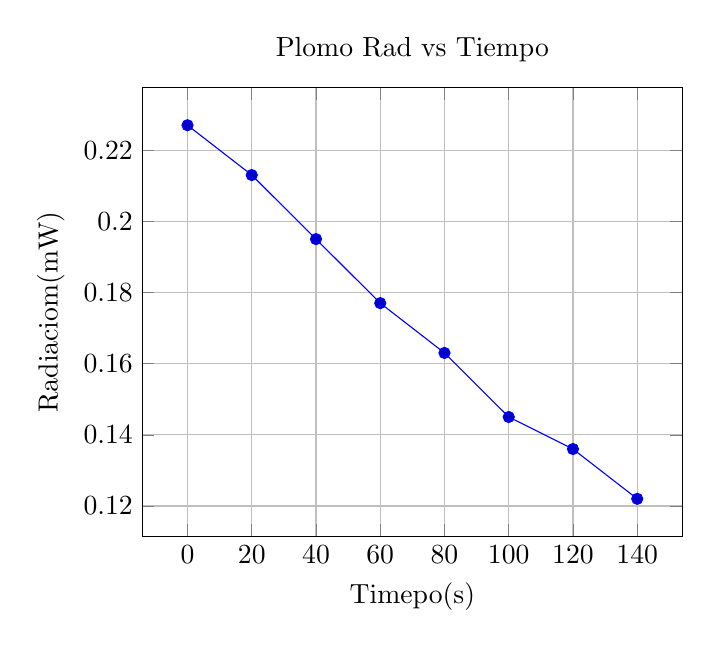
\begin{tikzpicture}
    \begin{axis}[
        xlabel={Timepo(s)},
        ylabel={Radiaciom(mW)},
        title={Plomo Rad vs Tiempo},
        grid=major,
        legend pos=north west
    ]
    \addplot coordinates {
      (0,0.227) (20,0.213 ) (40,0.195) (60,0.177) (80,0.163) (100,0.145) (120,0.136) (140,0.122)
    };
    \end{axis}
\end{tikzpicture}
\end{document}
